\documentclass[12pt]{article}

\usepackage[english]{babel}
\usepackage[utf8]{inputenc}
\usepackage{fancyhdr}

\usepackage[margin=1in]{geometry}
\usepackage{pgf}
\usepackage{pgfplots}
\usepackage{siunitx}
\usepackage{tikz}
\usepackage{float}
\usepackage{amsmath}

\usetikzlibrary{scopes}
\usetikzlibrary{angles,quotes}
\usetikzlibrary{calc}
\pgfplotsset{compat=1.5}

\begin{document}
\sisetup{per-mode=symbol}

\begin{titlepage}
    \begin{center}
        \vspace*{1cm}
        \textbf{Collisions}

        \vspace{0.5cm}
        Lab: 07

        \vspace{1cm}

        \textbf{Jaden Moore}

        \vfill

        Orange Coast College\\
        Physics A185L\\
        October 17th, 2020

    \end{center}
\end{titlepage}

\pagestyle{fancy}
\fancyhf{}
\setlength{\headheight}{15pt}
\lhead{Collisions}
\rhead{Lab: 07}
\cfoot{\thepage}

\section{Introduction}
In this lab, we discuss whether the total linear momentum in a system consisting of two masses and a spring is conserved throughout its motion. The initial setup of the system is that of the two masses positioned on either side of a compressed spring. That is, the compressed spring is in between the two masses. We then analyze the motion of the system as the spring decompresses back into its resting position and determine whether the total linear momentum of the system is conserved.

\section{Conservation Of Linear Momentum}
The law of conservation of momentum states that when there are no external forces acting on a system, then the linear momentum of the system remains constant throughout its motion. That is, when $F_\text{ext} = 0$ then, $P_i = P_f$. Consider the following setup of two masses and a spring, such that:

\begin{figure}[H]
    \centering

    \caption[10pt]{A system of two masses and a spring}

    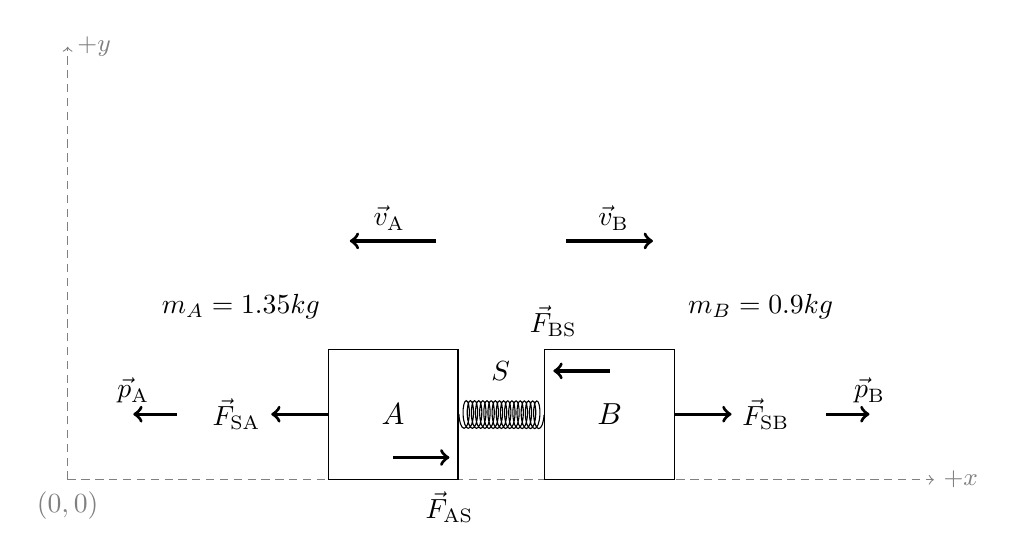
\begin{tikzpicture}[scale=1.1]
        \begin{scope}

            {[densely dashed,gray,font=\small,->]
                \draw (0,0) -- (0,5) node[right] {$+y$};
                \draw (0, 0) -- ++(10,0) node[right] {$+x$};
            }

            \node[gray] (origin) at (0, -0.3) {$(0, 0)$};

            % Mass A
            \node[] (l1) at (2, 2) {$m_A=1.35kg$};
            \node[rectangle,draw,color=black,fill=white,minimum size=1.5cm,transform shape,anchor=south west] (A) at (3,0) {$A$};

            \draw[very thick,->] (A.west) -- ++(-0.65,0) node[left] {$\vec{F}_\text{SA}$};

            \draw[very thick,->] ($(A)+(0,-0.5)$) -- ++(0.65,0) node[below, shift={(0,-0.3)}] {$\vec{F}_\text{AS}$};

            \draw[very thick,->] ($(A)+(0.5,2)$) -- ++(-1,0) node[above, shift={(0.5,0)}] {$\vec{v}_\text{A}$};

            \draw[very thick,->] ($(A)+(-2.5,0)$) -- ++(-0.5,0) node[above, shift={(0,0)}] {$\vec{p}_\text{A}$};


            % Spring 
            \node[] (l3) at (5, 1.25) {$S$};
            \draw[decoration={aspect=0.3, segment length=1.5, amplitude=5,coil},decorate] (5.5,0.75) -- (A);


            % Mass B
            \node[] (l1) at (8, 2) {$m_B=0.9kg$};
            \node[rectangle,draw,color=black,fill=white,minimum size=1.5cm,transform shape,anchor=south west] (B) at (5.5,0) {$B$};

            \draw[very thick,->] (B.east) -- ++(0.65,0) node[right] {$\vec{F}_\text{SB}$};

            \draw[very thick,->] ($(B)+(0,0.5)$) -- ++(-0.65,0) node[above, shift={(0,0.3)}] {$\vec{F}_\text{BS}$};

            \draw[very thick,->] ($(B)+(-0.5,2)$) -- ++(1,0) node[above, shift={(-0.5,0)}] {$\vec{v}_\text{B}$};

            \draw[very thick,->] ($(B)+(2.5,0)$) -- ++(0.5,0) node[above, shift={(0,0)}] {$\vec{p}_\text{B}$};

        \end{scope}
    \end{tikzpicture}
\end{figure}

In this case, The forces acting on masses $A$ and $B$ are a direct result of Newton's third law and thus are considered internal forces. That is, there are no external forces acting on the system. Because all the forces acting on the masses are internal and there are no external forces, we can see that the total linear momentum of the system is constant throughout time because the sum of the forces acting in the system is zero.

Furthermore, we can also conclude that the total energy in the system in its initial state is equal to the potential energy within the spring because the spring is compressed and the velocity of the two masses is zero, thus no kinetic energy exists in the masses initially. The force of a spring is considered conservative because the work done by the force is only determined by the final position of the stretch or compression of the spring, rather than the path taken to obtain the stretch or compression. Thus, all the forces in the system are conservative.

\paragraph{}

Consider that at 0.22 seconds into the motion of Figure 1, the spring $S$ has fully decompressed and the velocity $\vec{v}$ of the masses $A$ and $B$ due to the decompression is no longer zero, and the velocity is constant. Using one dimensional kinematics, we can determine the individual velocity $\vec{v}$ of the masses by taking the position of the masses some time after the velocity has become constant. The position of mass $A$ at $0.22$ seconds is taken to be $x_0 = -0.42 m$. The position of mass $A$ $0.08$ seconds after $x_0$ is taken to be $X_f = -0.50m$. Using the following kinematic equation:

\begin{equation} \label{eq1}
    x_f - x_0= + \vec{v_0}t + \frac{1}{2}at^2
\end{equation}

From equation 1, We have:

\begin{equation*}
    \begin{split}
        \SI{-0.50}{m} - (\SI{-0.42}{m}) & = \vec{v_A}(\SI{0.08}{s}) + \frac{1}{2}(0)(\SI{0.08}{s})^2 \\
        \SI{-0.08}{m} & = \vec{v_A}(\SI{0.08}{s}) \\
        \vec{v}_A & = \SI{-1.0}{m/s}
    \end{split}
\end{equation*}

In this case, the constant velocity of mass $A$ 0.22 seconds into the motion is $\SI{-1.0}{m/s}$. The same process can be applied to mass $B$, such that:

\begin{equation*}
    \begin{split}
        \SI{0.55}{m} - (\SI{0.43}{m}) & = \vec{v_B}(\SI{0.08}{s}) + \frac{1}{2}(0)(\SI{0.08}{s})^2 \\
        \SI{0.12}{m} & = \vec{v_B}(\SI{0.08}{s}) \\
        \vec{v}_B & = \SI{1.5}{m/s}
    \end{split}
\end{equation*}

We can then use the relationship between mass and velocity to identify the linear momentum of the individual masses. The linear momentum of any mass can be described such that:

\begin{equation} \label{eq2}
    \vec{p} = m\vec{v}
\end{equation}

Using equation 2 for masses $A$ and $B$, we have:

\begin{equation*}
    \begin{split}
        \vec{p}_A & = (\SI{1.35}{kg})(\SI{-1.0}{m/s}) = \SI{-1.35}{\kilogram\metre\per\second} \\
        \vec{p}_B & = (\SI{0.90}{kg})(\SI{1.5}{m/s}) = \SI{1.35}{\kilogram\metre\per\second}
    \end{split}
\end{equation*}

Since the spring is considered to be of negligible mass, the sum of the linear momentum of masses $A$ and $B$ is equal to the total linear momentum of the system at any moment in time. This also means that the initial potential energy from the spring that was used to propel the masses is now equivalent to the sum of the kinetic energy of the masses because the energy is never lost. From summing the linear momentum of the masses, we get that:

\begin{equation*}
    \vec{p}_\text{total} = (\vec{p}_A + \vec{p}_B) = \SI{0}{\kilogram\metre\per\second}
\end{equation*}

That is, the total linear momentum of the system at any moment in time is equal to zero. This makes intuitive sense even at $t = 0$ because nothing is moving, and it also makes intuitive sense at $t = 0.22$ seconds because the masses are moving with equal momentum, but in opposite directions, thus keeping the total linear momentum equal to zero.

\paragraph{}

Furthermore, if we consider the net force acting on the system as a whole, from Newton's third law, we can intuitively determine whether the total linear momentum is conserved. Consider that if the sum of the forces act on the system as a whole is zero, then the total linear momentum is conserved, such that:

\begin{equation}
    \sum{}{}\vec{F} = \vec{F}_\text{SA} + \vec{F}_\text{AS} + \vec{F}_\text{SB} + \vec{F}_\text{BS} = 0
\end{equation}

From Newton's third law and an analysis of Figure 1,  we get equation 3 to be true.

\section{Conclusion}
We concluded that by Newton's third law, the forces acting on the masses in Figure 1 are all internal. Thus, by the law of conservation of linear momentum, the total linear momentum of the system should be constant throughout its entire motion. We found the sum of the linear momentum of the individual masses after the spring was released to be $\SI{0}{\kilogram\metre\per\second}$, which represents the total linear momentum of the system at any other point in time. This makes intuitive sense because at $t = 0$ seconds, where nothing in the system is moving, the linear momentum of the system can simply be physically observed to be $\SI{0}{\kilogram\metre\per\second}$. From this, and the fact that the net force of the system is zero determined by Newton's third law, we can conclude that the results from the analysis supports the conclusion that momentum is conserved in the system presented in Figure 1.
\end{document}
